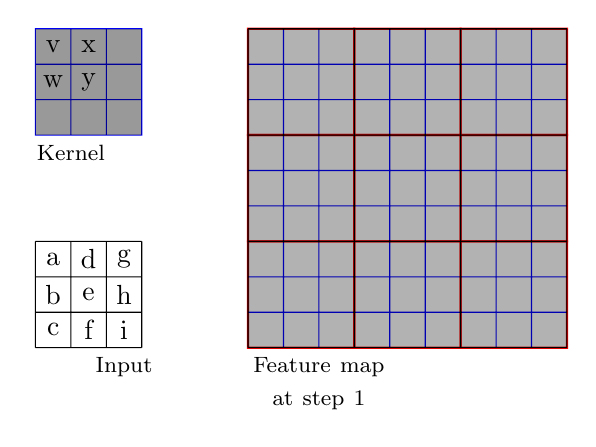
\begin{tikzpicture}
\begin{scope}[transparency group]
\begin{scope}[blend mode=multiply]

%stride 1
%kernel
%kernel
\draw [thin, draw=blue, fill=black!40!white,scale = .45] (-1,5) rectangle (2,8) grid (-1,5);
%kernel label
\draw [scale=.45,below] node at (0,5)  {\footnotesize Kernel};
%kernel components
\draw [scale=.45] node at (-0.5,7.5) {v};
\draw [scale=.45] node at (-0.5,6.5) {w};
\draw [scale=.45] node at (0.5,7.5)  {x};
\draw [scale=.45] node at (0.5,6.5)  {y};
%%step 1 equation
%\draw [scale=.45] node [text width=2cm,align=center] at (6,7) {\footnotesize \(o=(\mathbf{a}*v+0*w+0*x+0*y\)};
%%step 2 equation
%\draw [scale=.45] node [text width=2cm,align=center] at (12.5,7) {\footnotesize \(p=0*v+0*w+\mathbf{d}*x+0*y\)};
% input
%\draw [thick, draw=black, fill=black!40!white,scale = .45] (-1,2) rectangle (1,4);
%\draw [thick, draw=black, fill=black!40!white,scale = .45] (0,2) rectangle (2,4);
\draw [thin, draw=black,scale=.45] (-1,-1) grid  (2,2) node at (1.5,-1)[below] {\footnotesize Input};
% step 1 featuremap
%\draw [thick, draw=black, fill=black!40!white,scale = .45] (5,2) rectangle  (6,3);
\draw [thin, draw=blue,scale = .45] (5,-1) grid  (14,8) node at (7,-1) [below,text width=2cm,align= center] {\footnotesize Feature map at step 1};
%step 2 featuremap
%\draw [thick, draw=black, fill=black!40!white,scale = .45] (11,2) rectangle  (12,3);
%\draw [thick, draw=black,scale = .45] (10,-1) grid  (14,3) node at (12,-1) [below,text width=2cm,align= center] {\footnotesize Feature map at step 1};
%%draw arrows
%\draw [scale=.45,thick,arrow] (0,4)  to [bend angle=70, bend left] (5.5,3);
%\draw [scale=.45,thick,arrow] (1,4)  to [bend angle=40, bend left] (11.5,3);
%%	%draw step
%\draw [scale=.45] node[rotate=-40]   at (5.3,4.4) {\footnotesize Step 1};
%\draw [scale=.45] node[rotate=-40]   at (10.7,4.4) {\footnotesize Step 2};
%draw abc step 1
%draw abc step 1
\draw [scale=.45] node at (-.5,1.5) {a};
\draw [scale=.45] node at (-.5,0.5) {b};
\draw [scale=.45] node at (-.5,-.5) {c};
\draw [scale=.45] node at (0.5,1.5) {d};
\draw [scale=.45] node at (0.5,0.5) {e};
\draw [scale=.45] node at (0.5,-.5) {f};
\draw [scale=.45] node at (1.5,1.5) {g};
\draw [scale=.45] node at (1.5,0.5) {h};
\draw [scale=.45] node at (1.5,-.5) {i};

\foreach \i in {-1,2,5}
\foreach \j in {5,8,11}
\draw [thick, draw=red, fill=black!30!white,scale = .45] (\j,\i) rectangle  (\j+3,\i+3);

\end{scope}
\end{scope}
\end{tikzpicture}
